%!TEX root = ../main.tex

\chapter{L'imagerie \glsentryshort{stem} : présentation et problématiques}
\label{ch-chapter_1}

    \dochaptoc
    \graphicspath{{img/chapitre2/}}

    \section{Présentation de la microscopie \glsentryshort{stem}}

    L'ensemble du travail de thèse présenté dans ce manuscrit se base sur des données issues d'un système de microscopie appelé Microscope \'Electronique en Transmission à Balayage ou encore \acf{stem}\glsunset{stem}. Ce système utilise un faisceau d'électrons pour illuminer un échantillon et obtenir ainsi un agrandissement de la zone à étudier, il s'agit donc d'un microscope électronique. Nous allons commencer par positionner le \gls{stem} au sein de la microscopie électronique pour ensuite décrire plus précisément son fonctionnement.

    \subsection{La microscopie électronique}

    Un microscope électronique se compose classiquement d'une source d'électrons (aussi appelé canon), de lentilles électromagnétiques permettant de focaliser le faisceau de particules sur l'échantillon et d'un détecteur. En définitive, les types de microscopes électroniques se différencient par la façon dont l'échantillon est illuminé et par la position du détecteur. Nous y trouvons donc :
    \begin{itemize}
    	\item la microscopie électronique en transmission (aussi appelée \gls{tem}) pour laquelle le faisceau d'électrons illumine l'ensemble de l'échantillon et le traverse pour être ensuite analysé,
    	\item la microscopie \gls{stem} pour laquelle le faisceau d'électrons est focalisé sur un point de l'échantillon et le traverse pour être ensuite analysé,
    	\item la microscopie électronique à balayage (aussi appelée \gls{sem}) pour laquelle le faisceau d'électrons est focalisé sur un point de l'échantillon et le détecteur positionné en amont capte des électrons secondaires s'étant déviés.
    \end{itemize}
    La \cref{fig-chap2-micros-electron} propose un schéma simplifié de ces configurations. Chacune de ces modalités permettent l'acquisition d'une image contrastée 2D qui est une représentation agrandie de l'échantillon.

    \begin{figure*}[t!]
       	\centering
       	\subfigure[Légende]{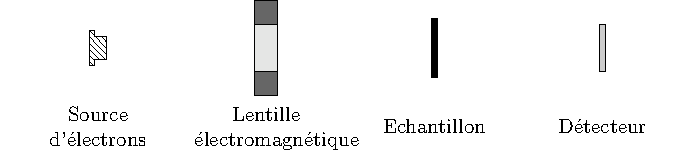
\includegraphics[]{img/chapitre2/figure1/subfig-a/electronic-legend.pdf}
       	}\\
       	\subfigure[Le microscope \gls{tem}]{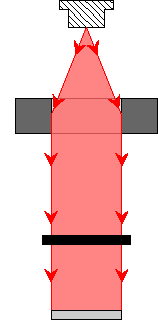
\includegraphics[]{img/chapitre2/figure1/subfig-b/electronic-tem.pdf}}
       	\hspace*{2cm}
       	%
       	\subfigure[Le microscope \gls{stem}]{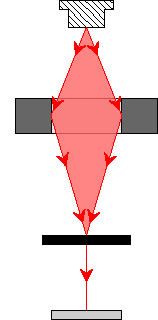
\includegraphics[]{img/chapitre2/figure1/subfig-c/electronic-stem.pdf}}
       	\hspace*{2cm}
       	%
       	\subfigure[Le microscope \gls{sem}]{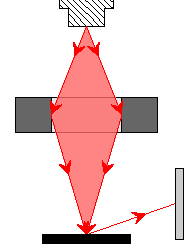
\includegraphics[]{img/chapitre2/figure1/subfig-d/electronic-sem.pdf}}
       	%
           \vspace{1em}
       	\caption{Schéma de principe des différents types de microscopie électronique.%
               \protect\label{fig-chap2-micros-electron}}
   \end{figure*}

    Les microscopes \gls{stem} et \gls{sem} se différencient du \gls{tem} puisque le faisceau balaye l'échantillon ligne par ligne au lieu de l'illuminer entièrement. Il en résulte que ces premiers sont destinés principalement à la \emph{spectroscopie}, i.e. à l'acquisition d'un spectre pour chaque position spatiale. Les données peuvent alors être perçues comme un cube ayant deux directions spatiales et une direction spectrale. Des applications classiques de ces systèmes sont la détection et cartographie d'éléments chimiques présents dans l'échantillon (cf. \cref{sec-exploitation-eels}). Le \gls{tem} est davantage utilisé en \emph{imagerie} pour représenter l'échantillon sans analyse chimique possible.

    La suite de ce manuscrit se focalisera sur la microscopie \gls{stem} qui est le centre de notre étude. C'est pourquoi le principe physique de la microscopie en transmission va être évoquée et les modalités d'acquisition classiques vont être présentées. A cette fin, un schéma plus détaillé de ce système et de ses modalités d'acquisition est donné en \cref{fig-chap2-stem-detail} et servira de support. D'autre part, le contenu technique de ce chapitre s'inspire du livre de Egerton~\cite{egerton2011electron} et nous renvoyons les lecteurs curieux à cet ouvrage pour de plus amples informations.

    \begin{figure*}[htbp]
    	\centering
    	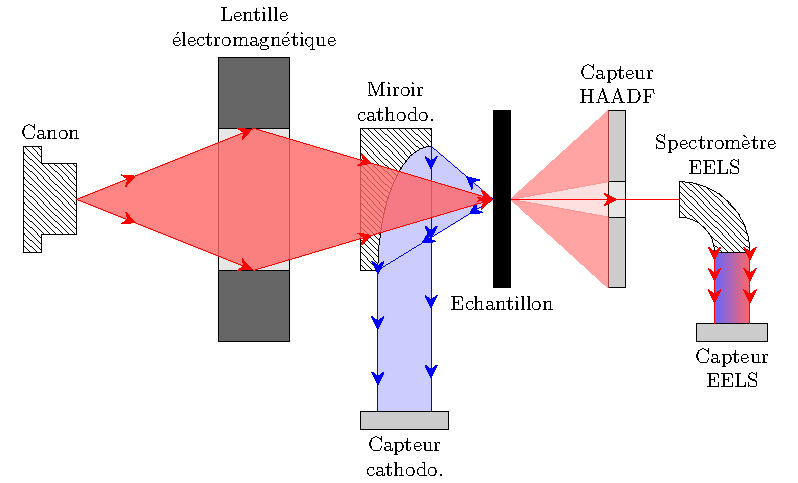
\includegraphics[]{img/chapitre2/figure2/stem-detail.pdf}
    	\caption{Un schéma de principe détaillé du \gls{stem}.
        	\protect\label{fig-chap2-stem-detail}}
    \end{figure*}

    \subsection{Principe de la microscopie en transmission}

    La microscopie en transmission étudie les interactions physiques entre un faisceau d'électron et la matière qu'il traverse. Pour ce faire, un canon fournit une certaine énergie cinétique à un faisceau d'électrons, celui-ci est alors focalisé en un point de l'échantillon à l'aide de lentilles électromagnétiques. Afin que ce faisceau \emph{traverse} l'échantillon, plusieurs conditions doivent être réunies :
    \begin{enumerate}[label=(\alph*)]
    	\item l'énergie cinétique des électrons doit être suffisante (typiquement 100keV),
    	\item l'échantillon doit être suffisamment fin (typiquement 100nm pour un faisceau de 100keV).
    \end{enumerate}
    Dans ces conditions, les électrons traversent l'échantillon sans subir d'absorption ni de réflexion notoire. A noter qu'il est nécessaire de faire le vide dans le corps du microscope afin d'éviter toute collision entre le faisceau et les molécules constituant notre atmosphère. Dès lors, des interactions électron-atome vont avoir lieu \emph{au sein de l'échantillon}, séparés grossièrement en trois catégories : diffusion élastique, diffusion inélastique en couche électronique basse et diffusion inélastique en couche électronique haute.

    La diffusion élastique se caractérise par une interaction sans perte d'énergie cinétique. Elle fait intervenir une répulsion électrostatique entre le noyau électronique fortement chargé et l'électron incident. Le champ électrostatique est puissant au c\oe{}ur de l'atome et l'électron incident est d'autant plus dévié de sa trajectoire qu'il passe à proximité du noyau (cf \cref{fig-chap2-interactions-a}). Cela dit, la majorité des électrons traversent l'atome suffisamment loin du noyau pour être peu déviés et l'angle de diffusion n'est généralement que de quelques degrés (10-100 mrad).

    Une diffusion inélastique, quant à elle, se caractérise par une perte d'énergie cinétique. L'énergie perdue permet alors de déplacer un ou plusieurs électrons appartenant à l'atome sur des couches électroniques plus hautes. Dans le cas où l'électron atomique se situe en couche électronique basse, l'énergie transférée correspond à la différence de niveau d'énergie entre les niveaux de départ et d'arrivée (cf \cref{fig-chap2-interactions-b}). Dans le cas où l'électron transféré se situe en couche électronique haute, la quantité d'énergie transférée peut prendre un continuum de valeur puisque l'électron se déplace au sein d'une bande de valence (cf \cref{fig-chap2-interactions-c}).

    Il en résulte que les électrons traversant l'échantillon sont à la fois déviés de leur trajectoire (possiblement fortement) et ralentis dû à un transfert d'énergie. Les modalités d'acquisition du \gls{stem} se basent sur la détection de ces deux effets.

    \begin{figure}
    	\centering
    	\subfigure[Diffusion élastique]{
    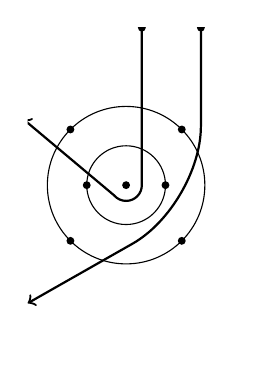
\begin{tikzpicture}[scale=0.5]
        \clip (-2.5, -4) rectangle (2.5, 4);
        \coordinate (O) at (0, 0);
        \coordinate (A) at (0.4, 4);
        \coordinate (B) at (1.9, 4);

        % Circles
        \draw (O) circle (1cm);
        \draw (O) circle (2cm);

        % Central atom
        \fill[black] (O) circle (0.1cm);

        % Atoms on layers # 1
        \fill[black] (0:1) circle (0.1cm);
        \fill[black] (180:1) circle (0.1cm);

        % Atoms on layers # 2
        \fill[black] (45:2) circle (0.1cm);
        \fill[black] (90+45:2) circle (0.1cm);
        \fill[black] (180+45:2) circle (0.1cm);
        \fill[black] (270+45:2) circle (0.1cm);

        % Incident atoms
        \fill[black] (A) circle (0.1cm);
        \fill[black] (B) circle (0.1cm);

        \draw[->, thick ] (A) -- (0.4, 0) arc (0:-140:0.4) -- ++ (140:3);
        \draw[->, thick, rounded corners=1cm ] (B) -- ++(0, -4.5) -- (-2.5, -3);

    \end{tikzpicture}
    \label{fig-chap2-interactions-a}
}\quad
\subfigure[Diffusion inélastique en couche électronique basse]{
    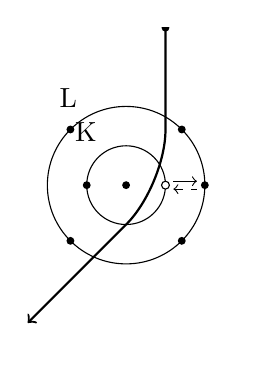
\begin{tikzpicture}[scale=0.5]
        \clip (-2.5, -4) rectangle (2.5, 4);

        \coordinate (O) at (0, 0);
        \coordinate (A) at (1, 4);

        % Circles
        \draw (O) circle (1cm);
        \draw (O) circle (2cm);

        % Central atom
        \fill[black] (O) circle (0.1cm);

        % Atoms on layers # 1
        \filldraw[draw=black, fill=white] (0:1) circle (0.1cm);
        \fill[black] (180:1) circle (0.1cm);
        \draw (120:1) node [above left] {K};

        % Atoms on layers # 2
        \fill[black] (45:2) circle (0.1cm);
        \fill[black] (90+45:2) circle (0.1cm);
        \fill[black] (180+45:2) circle (0.1cm);
        \fill[black] (270+45:2) circle (0.1cm);
        \draw (120:2) node [above left] {L};

        % Incident atoms
        \fill[black] (A) circle (0.1cm);
        \draw[->, thick, rounded corners=0.7cm ] (A) -- (1, 0) -- (-2.5, -3.5);

        % Other atom and arrows
        \fill[black] (2, 0) circle (0.1cm);
        \draw [->] (1.2, 0.1) -- ++ (0.6, 0);
        \draw [<-, dashed] (1.2,- 0.1) -- ++ (0.6, 0);

    \end{tikzpicture}
    \label{fig-chap2-interactions-b}
}\quad
\subfigure[Diffusion inélastique en couche électronique haute]{
    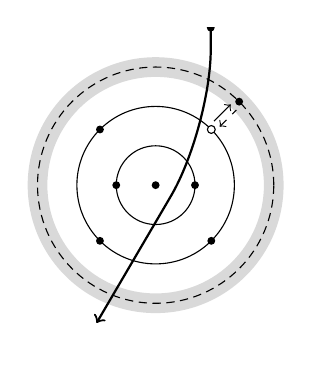
\begin{tikzpicture}[scale=0.5]
        \clip (-3.25, -4) rectangle (3.25, 4);

        \coordinate (O) at (0, 0);
        \coordinate (A) at (1.4, 4);

        % Circles
        \draw (O) circle (1cm);
        \draw (O) circle (2cm);

        % Central atom
        \fill[black] (O) circle (0.1cm);

        % Atoms on layers # 1
        \fill[black] (0:1) circle (0.1cm);
        \fill[black] (180:1) circle (0.1cm);

        % Atoms on layers # 2
        \filldraw [draw=black, fill=white] (45:2) circle (0.1cm);
        \fill[black] (90+45:2) circle (0.1cm);
        \fill[black] (180+45:2) circle (0.1cm);
        \fill[black] (270+45:2) circle (0.1cm);

        % Layer # 3
        \fill [black!15, even odd rule] (O) circle (3.25cm) circle (2.75cm);
        \draw [densely dashed] (O) circle (3cm);

        % Incident atoms
        \fill[black] (A) circle (0.1cm);
        \draw[->, thick, rounded corners=1cm ] (A) -- ++(0, -2.55) -- (-1.5, -3.5);

        % Other atom and arrows
        \fill [black] (45:3) circle (0.1cm);
        \draw [->, rotate=45] (2.2, 0.1) -- ++ (0.6, 0);
        \draw [<-, dashed, rotate=45] (2.2,- 0.1) -- ++ (0.6, 0);

    \end{tikzpicture}
    \label{fig-chap2-interactions-c}
}

        \vspace{1em}
    	\caption{Une représentation classique de la diffusion électronique inspirée de~\cite{egerton2011electron}.%
            \protect\label{fig-chap2-interactions}}
    \end{figure}


    \subsection{Les modalités d'acquisition en microscopie \glsentryshort{stem}}

    Le \gls{stem} permet entre autre trois modalités d'acquisition : la cathodoluminescence, l'acquisition fond noir angulaire à grand angle (ou encore \gls{haadf}) et la spectroscopie par perte d'énergie (ou encore \gls{eels}). La \cref{fig-chap2-stem-detail} sert de support pour situer ces instruments dans le \gls{stem}.

    \paragraph*{Cathodoluminescence} Pour certains échantillons, le faisceau incident produit un phénomène de fluorescence dépendant de la nature de l'échantillon et de ses défauts. La technique consistant à acquérir ce signal et à l'étudier s'appelle \emph{la cathodoluminescence}. Le flux lumineux est recueilli à l'aide d'un miroir situé en amont de l'échantillon puis envoyé vers un spectromètre qui procède à l'analyse.

    \paragraph{\gls{haadf}} Le faisceau incident se situe dans l'axe optique de l'appareil et une grande partie des électrons traversent l'échantillon en demeurant dans cet axe, la diffusion élastique est alors négligeable. Néanmoins, une partie des électrons sont significativement déviés de l'axe optique en sortie.  Un capteur annulaire placé en aval de l'échantillon capte ces électrons et délivre un signal proportionnel. Cette technique appelée \gls{haadf} permet de fournir une image 2D de l'échantillon. Un exemple d'acquisition \gls{haadf} est fournie à la \cref{fig-chap2-haadf-ex}.

    \begin{figure}%[htbp]
    	\centering
    	\subfigure[\label{fig-chap2-haadf-ex-a}Acquisition basse-résolution]%
            {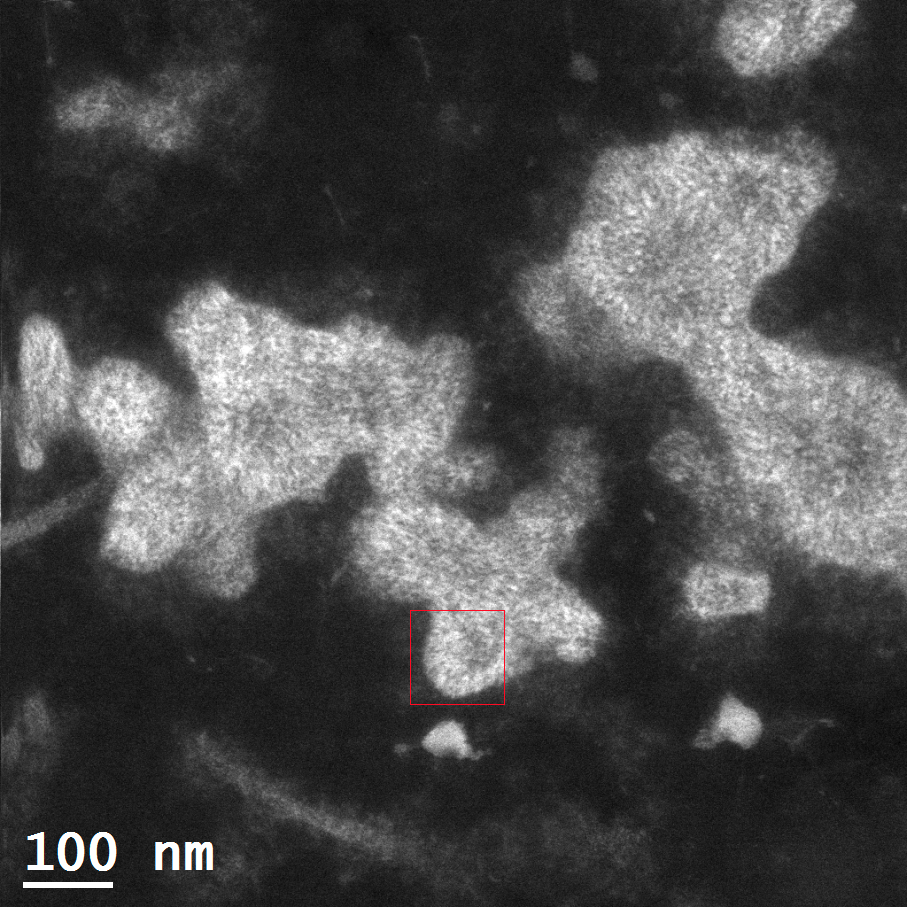
\includegraphics[height=0.25\textwidth]{img/chapitre2/figure4/haadf-LR.png}}
        \hspace{1em}
        \subfigure[\label{fig-chap2-haadf-ex-b}Acquisition haute-résolution]%
            {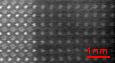
\includegraphics[height=0.25\textwidth]{img/chapitre2/figure4/haadf-HR-sc.png}}
     	%
        \caption{\protect\label{fig-chap2-haadf-ex}Exemples d'acquisitions \gls{haadf}. L'acquisition basse-résolution~\protect\subref{fig-chap2-haadf-ex-a} est à échelle micrométrique  tandis que l'acquisition haute-résolution~\protect\subref{fig-chap2-haadf-ex-b} est à échelle nanométrique.}
     \end{figure}


    \paragraph*{\gls{eels}} Comme expliqué précédemment, une quantité importante des électrons traversant l'échantillon  perdent une partie de leur énergie initiale. Afin d'étudier cela, le faisceau demeuré dans l'axe optique frappe un spectromètre séparant les électrons en fonction de leur énergie. Une caméra CCD permet de compter, pour chaque position sur l'échantillon, la quantité d'électrons ayant conservé une énergie donnée. \`A chaque position spatiale correspond alors un spectre de perte d'énergie, les images \gls{eels} sont d'ailleurs également appelées \emph{spectre-image}. La microscopie \gls{eels} constitue le centre de cette étude, c'est pourquoi nous allons détailler ces données et leurs propriétés dans la section suivante.


    \section{Propriétés des données \glsentryshort{eels}}\label{sec-prop-eels}

    \begin{figure}[t]
        \centering
        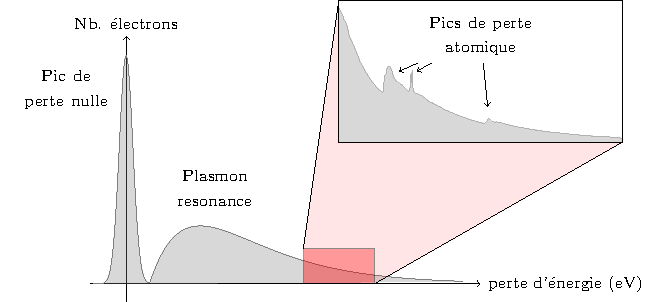
\includegraphics[]{img/chapitre2/figure5/eels-spectrum-shape.pdf}
        \caption{Représentation d'un spectre \gls{eels}.}
        \label{fig-chap2-eels-spectrum-shape}
    \end{figure}

    \paragraph{Caractéristiques spectrales} La forme générique d'un spectre \gls{eels} est représenté à la \cref{fig-chap2-eels-spectrum-shape}. Celui-ci représente le nombre d'électrons ayant traversé l'échantillon en fonction de l'énergie perdue après la traversée (on parle de \emph{canal} pour désigner l'indice associé à une perte d'énergie). Il se compose de trois parties :
    \begin{itemize}
    	\item un pic de perte nulle qui correspond à l'ensemble des électrons ayant traversé l'échantillon sans interagir avec lui, et donc sans avoir perdu d'énergie,
    	\item un pic plus étalé correspondant à une excitation collective de la bande de valence,
    	\item une zone d'intérêt où un ensemble de pics caractéristiques (appelés \emph{seuils}) émergent du fond décroissant.
    \end{itemize}
    \`A noter que le pic de pertes nulles permet de calibrer le zéro de l'axe des abscisses après acquisition. \emph{L'information utile est porté par la position, la forme et l'amplitude des seuils}. En effet, la position d'un seuil permet de déterminer l'élément présent dans l'échantillon tandis que son amplitude nous renseigne sur son abondance pour chaque position spatiale. Enfin, la forme du seuil peut varier suivant la configuration électronique de l'élément étudié.
    %
    Pour servir d'exemple, les seuils généralement rencontrés dans nos données se situent à des pertes d'énergie de l'ordre de 500 à 1000 eV (pour rappel, une énergie typique en amont de l'échantillon est 100keV).
    %
    Un exemple réel de spectre est donné en \cref{fig-chap2-eels-real-spectra-figure}.


    \begin{figure}[htbp]
        \centering
        \subfigure[La position des spectres]{
            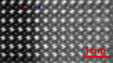
\includegraphics[width=0.4\textwidth]{img/chapitre2/figure6/eels_spectra_haadf-sc.png}
            \label{fig-chapitre2-real-eels-haadf}
        }\\
        \subfigure[Les spectres pour les trois positions]{
            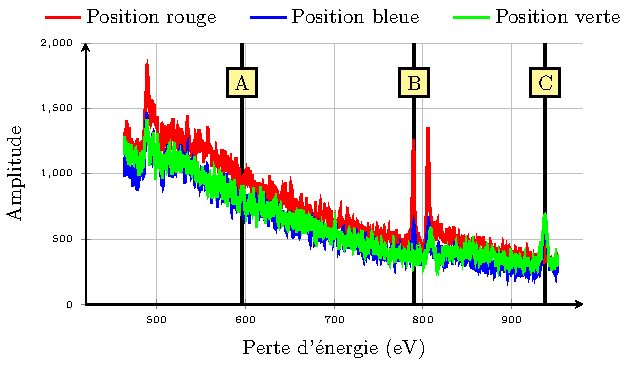
\includegraphics[]{img/chapitre2/figure6/eels_spectra.pdf}
            \label{fig-chapitre2-real-eels-spectra}
        }\\
        %
        \subfigure[Bande A]{% $\mathrm{O-K}$
            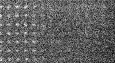
\includegraphics[width=0.3\textwidth]{img/chapitre2/figure6/eels_spectra_band_410.png}
            \label{fig-chapitre2-real-eels-bandA}
        }
        \hspace*{0.5cm}
        %
        \subfigure[Bande B ($\mathrm{La-M}_{4, 5}$)]{
            
\includegraphics[width=0.3\textwidth]{img/chapitre2/figure6/eels_spectra_band_1001.png}
            \label{fig-chapitre2-real-eels-bandB}
        }
        \hspace*{0.5cm}
        %
        \subfigure[Bande C ($\mathrm{Nd-M}_{4, 5}$)]{
            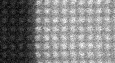
\includegraphics[width=0.3\textwidth]{img/chapitre2/figure6/eels_spectra_band_1465.png}
            \label{fig-chapitre2-real-eels-bandC}
        }

        \caption{Exemple réel d'image \gls{eels}. La Figure~\protect\subref{fig-chapitre2-real-eels-haadf} représente l'image \gls{haadf} de l'acquisition et trois positions en rouge, bleu et vert. Les spectres acquis en ces trois positions sont représentés à la figure~\protect\subref{fig-chapitre2-real-eels-spectra}. Enfin, les données spatiales à trois niveaux de perte d'énergie (notées A, B et C à la figure~\subref{fig-chapitre2-real-eels-spectra}) sont représentées aux figures~\subref{fig-chapitre2-real-eels-bandA} à \subref{fig-chapitre2-real-eels-bandC}. Les bandes B (resp. C) correspondent à la signature $\mathrm{La-M}_{4, 5}$ (resp. $\mathrm{Nd-M}_{4, 5}$) tandis que la bande A ne correspond à aucune signature.
            \protect\label{fig-chap2-eels-real-spectra-figure}}
    \end{figure}

    Plus précisément, l'effet d'un seuil ne se limite pas au pic puisque un biais positif persiste après le seuil. La courbe peut alors être décomposé en la somme d'un fond décroissant (généralement modélisé par une exponentielle décroissante) et de divers sauts, comme le montre la \cref{fig-decroissance-spectre}. Cette modélisation est la base des techniques de cartographie vues en \cref{sec-exploitation-eels}.

    \begin{figure*}
        \centering
        \subfigure[\label{fig-seuil-a}]{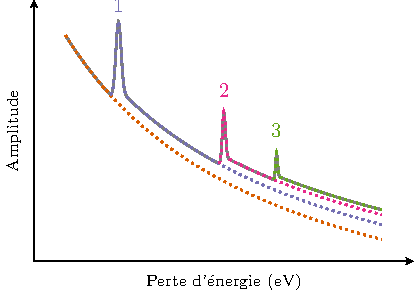
\includegraphics[]{img/chapitre2/figure6-bis/seuils.pdf}}
        \hspace{1em}
        \subfigure[\label{fig-seuil-b}]{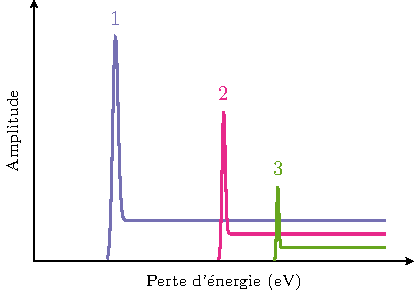
\includegraphics[]{img/chapitre2/figure6-bis/seuils-2.pdf}}
        \caption{Visualisation des effets de seuils successifs sur le spectre. La figure~\subref{fig-seuil-a} représente la forme d'un spectre constitué de trois seuils. Le fond décroissant est mis en évidence ainsi que le biais rémanent associé à chaque saut. La figure~\subref{fig-seuil-b} représente les effets isolés de chacun des trois seuils. Nous y distinguons le pic caractéristique de l'élément ainsi que le biais suivant chaque pic.
            \protect\label{fig-decroissance-spectre}}
    \end{figure*}


    \paragraph*{Caractéristiques spatiales} En microscopie, comme pour beaucoup de systèmes d'imagerie, la caractéristique principale est la résolution. En microscopie \gls{stem}, celle-ci est principalement limitée par la taille de la sonde électronique (typiquement 1~nm) et par les aberrations sphériques (un correcteur permet de descendre à 0.1~nm). D'autre part, la résolution est choisie par l'expérimentateur en fonction de la distance parcourue par la sonde entre deux acquisitions. Cependant, en imagerie \gls{eels}, la taille de l'image excède rarement $10^5$ pixels pour limiter le temps d'acquisition et éviter de détériorer l'échantillon (comme nous verrons plus loin). Par conséquent, deux situations apparaissent~:
    \begin{itemize}
        \item l'expérimentateur étudie des structures spatiales étendues (typiquement 100~nm) et est obligé de limiter la résolution, les images sont alors basse-résolution (cf. \cref{fig-chap2-haadf-ex-a}),
        \item l'expérimentateur étudie des réseaux atomiques très localisés (typiquement quelques nanomètres) et la résolution est limité par l'instrument, les images sont alors haute-résolution (cf. \cref{fig-chap2-haadf-ex-b}).
    \end{itemize}
    Enfin, il faut noter que la structure spatiale est plus ou moins visible selon le canal considéré dans l'image \gls{eels}. Par exemple, la \cref{fig-chapitre2-real-eels-bandA} correspond à une zone du spectre où aucun contraste n'apparaît clairement, il en résulte que l'image est fortement bruitée. A contrario, les images situées sur des seuils particuliers du spectre sont moins bruitées et mettent clairement en évidence la position des éléments concernés, comme pour les \cref{fig-chapitre2-real-eels-bandB,fig-chapitre2-real-eels-bandC}. Ainsi, l'utilisateur peut avoir une première idée de la cartographie des éléments étudiés, même si celle-ci est biaisée à cause de la contribution des seuils précédents (certains atomes apparaissent dans la \cref{fig-chapitre2-real-eels-bandA} du fait du seuil précédent la bande A, visible vers 500eV en \cref{fig-chapitre2-real-eels-spectra}). L'exploitation des données \gls{eels} sera approfondi dans la \cref{sec-exploitation-eels}.

    \paragraph*{Nature du bruit} Les sources de bruit sont multiples en imagerie \gls{eels}, mais le type de bruit le plus attendu est poissonien. Cela modélise tant la probabilité qu'un électron du faisceau subisse un certain nombre de diffusions inélastique au sein de l'échantillon~\cite[Section~4.1.1]{egerton2011electron} que la probabilité qu'une cellule du capteur reçoive un électron sur une période donnée. \`A cela s'ajoute un bruit gaussien dû à l'électronique d'acquisition.
    %
    En pratique, la nature du bruit est expérimentalement complexe à déterminer.
    %
    A ce bruit d'acquisition vient s'ajouter les instabilités spatiales de l'échantillon : celui-ci dérive au cours de l'acquisition dû à des variations de température, des mouvements d'air~\cite{zobelli2019spatial}. Ces déplacements ne sont pas visibles pour des images basse-résolution mais deviennent critiques à des échelles atomiques puisque le réseau atomique initialement aligné apparaît déformé, comme le montre la Figure~\ref{fig-drift}.
    %
    Enfin, des incertitudes de positionnement du faisceau s'ajoutent au cours de l'acquisition.

    \begin{marginfigure}
    	\centering
    	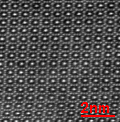
\includegraphics[width=0.7\textwidth]{img/chapitre2/figure7/drift-sc.png}
    	\caption{Un exemple de défaut en haute résolution : la dérive de l'échantillon. L'échantillonnage se fait ligne par ligne. On observe que, dans ce cas, l'échantillon dérivait sur la gauche, puis vers le haut. Il en résulte une déformation notable et préjudiciable du réseau.}
            %L'échantillon est un grenat de bismuth et de fer.}
    	\label{fig-drift}
    \end{marginfigure}


    \paragraph*{Redondance spectrale} L'imagerie \gls{eels} est un cas particulier d'imagerie hyperspectrale, dans les deux cas, il s'agit d'une acquisition spectroscopique. Les images rencontrées dans de nombreuses modalités incluant l'imagerie hyperspectrale et \gls{eels} sont connues pour être hautement corrélées spectralement~\cite{dobigeon_linear_2016, bioucas2012hyperspectral, dobigeon2012spectral}. Il en résulte que les données représentées dans un espace de dimension $N$ (où $N$ est le nombre de canaux) n'occupent pas indifféremment l'espace mais sont localisés dans une variété de dimension réduite. Celle-ci est non-linéaire par défaut, et une approximation linéaire est généralement réalisée par \gls{pca}. Une représentation de cette propriété est donnée à la \cref{fig-correlation}. L'analyse par \gls{pca} a plusieurs intérêts parmi lesquels le débruitage  et la réduction de la dimension des données \gls{eels}. En effet, les valeurs propres associées à l'\gls{pca} (représentée en \cref{fig-sub-pca-eigs}) sont généralement séparées en deux groupes suivant leur comportement : les premières de puissance\footnote{Il faut comprendre la puissance d'une composante principale comme la valeur propre associée à cette composante.} significativement supérieures et les autres de puissance semblable correspondant à la variance du bruit. Il en résulte que les données peuvent être considérées comme faible rang. Il s'agit là d'une propriété hautement intéressante qui sera utilisée dans la suite du manuscrit. Relevons enfin que les données peuvent être fortement débruités en seuillant l'\gls{pca}, c'est-à-dire en ne conservant que les premières composantes principales, puis en effectuant une rétro-projection.

    \begin{figure}[htb]
    	\centering
    	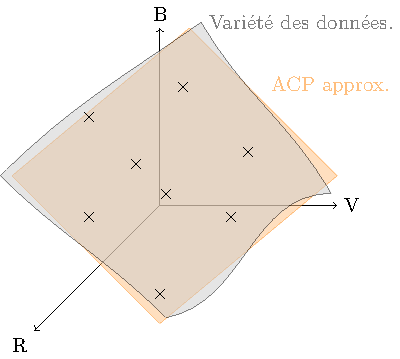
\includegraphics[]{img/chapitre2/figure8/redondance.pdf}
    	\caption{Une illustration de la redondance spectrale des données \gls{eels}. En considérant des spectres RVG (donc à 3 composantes), il est possible de les représenter dans l'espace. Or, les acquisitions (représentées ici par des points) n'occupent pas l'espace entier, mais se localisent plutôt à proximité d'une variété représentée en gris. L'analyse en composante principale permet d'obtenir une approximation \emph{linéaire} de la variété. Cet exemple considère une variété de dimension 2 dans un espace de dimension 3, mais cela se généralise pour des spectres de dimension $N$. Dans ces conditions, la variété est de dimension inférieure à $N$.
            \protect\label{fig-correlation}}
    \end{figure}


    \begin{figure}[htbp]
    	\centering
    	\subfigure[Evolution des valeurs propres associées à l'\gls{pca}]{
    		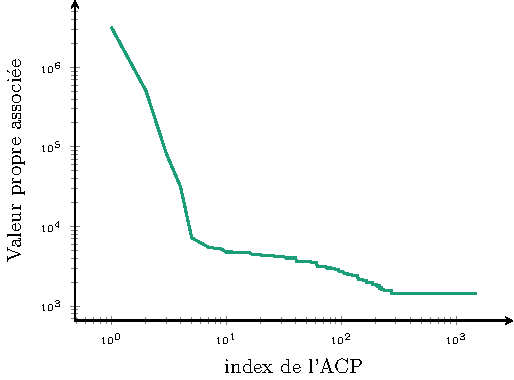
\includegraphics[]{img/chapitre2/figure9/PCA_eigs.pdf}
    		\label{fig-sub-pca-eigs}}
    	\\
    	\subfigure[Composante 0]{
    		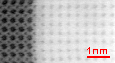
\includegraphics[width=0.28\textwidth]{img/chapitre2/figure9/PCA_map_0-sc.png}
    		\label{fig-sub-pca-comp0}
    	}\vspace{20pt}
    	\subfigure[Composante 1]{
    		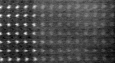
\includegraphics[width=0.28\textwidth]{img/chapitre2/figure9/PCA_map_1.png}}\vspace{20pt}
    	\subfigure[Composante 2]{
    		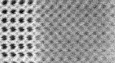
\includegraphics[width=0.28\textwidth]{img/chapitre2/figure9/PCA_map_2.png}}\\
    	\subfigure[Composante 3]{
    		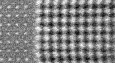
\includegraphics[width=0.28\textwidth]{img/chapitre2/figure9/PCA_map_3.png}}\vspace{20pt}
    	\subfigure[Composante 4]{
    		
\includegraphics[width=0.28\textwidth]{img/chapitre2/figure9/PCA_map_4.png}}\vspace{20pt}
    	\subfigure[Composante 5]{
    		
\includegraphics[width=0.28\textwidth]{img/chapitre2/figure9/PCA_map_5.png}
    		\label{fig-sub-pca-comp5}
    	}\\
    	%
    	\def\comp{mean}
    	\subfigure[Spectre moyen]{
    		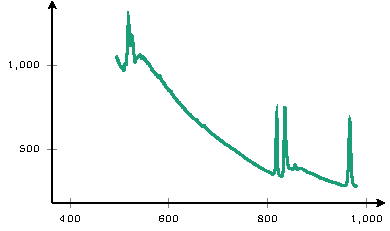
\includegraphics[]{img/chapitre2/figure9/PCA_spectra_1.pdf}
    		\label{fig-sub-pca-mean}}%
    	%
    	\def\comp{comp0}%
    	\subfigure[Première composante - spectre]{
    		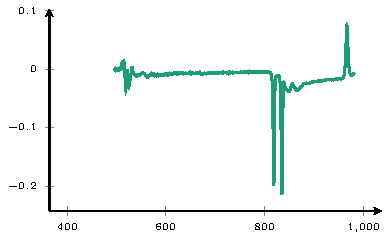
\includegraphics[]{img/chapitre2/figure9/PCA_spectra_2.pdf}
    		\label{fig-sub-pca-spectrum-0}}
    	%
    	\caption{L'analyse par \gls{pca} de données \gls{eels}. La figure~\subref{fig-sub-pca-eigs} représente l'évolution des valeurs propres associées à l'\gls{pca}. On observe, entre autres, que seules les 5 premières composantes sont vraiment significatives. Les figures \subref{fig-sub-pca-comp0} à \subref{fig-sub-pca-comp5} représentent la projection des données sur les spectres des composantes principales les plus puissantes. Le spectre moyen donné à la figure~\subref{fig-sub-pca-mean} est soustrait aux données avant d'appliquer l'\gls{pca}. Il en résulte que les spectres associés aux composantes principales sont dès lors bruitées, comme pour la composante 0 à la figure~\subref{fig-sub-pca-spectrum-0}.
            \protect\label{fig-ACP}} 
    \end{figure}


    %
    \section{Exploitation des données \glsentryshort{eels}}\label{sec-exploitation-eels}

    Comme expliqué précédemment, les données \gls{eels} présentent un intérêt tout particulier en cartographie d'éléments chimiques. Cette technique permet non seulement de cartographier la distribution spatiale des éléments, mais également de détecter des structures fines correspondant à des structures électroniques locales. Les images représentant la répartition de ces éléments sont appelés \emph{cartes d'abondances}. Deux méthodes sont classiquement utilisées~: la cartographie par séparation de composantes spectrales et les techniques de démélange.

    \subsection{Cartographie par séparation de composantes spectrales}

    Comme expliqué en \cref{sec-prop-eels}, un spectre \gls{eels} contient la contribution de plusieurs seuils successifs et d'un fond décroissant. Pour cartographier l'élément associé à un seuil, une méthode naïve consiste à intégrer le spectre autour du seuil pour chaque position spatiale et de représenter l'image obtenue. Néanmoins, le fond décroissant et la rémanence de seuils précédents biaise ce résultat, faisant apparaître des structures erronées dans les cartes d'abondance.

    Pour pallier ce problème, le fond décroissant et la rémanence des seuils précédents devront être soustrait avant d'intégrer le seuil d'intérêt. Pour illustrer cette méthode, considérons le spectre affiché en \cref{fig-carto-separation-a}, correspondant à une position spatiale donnée. Une zone de régression est choisie en amont du seuil (tout en restant proche du seuil) et une régression exponentielle est effectuée (cf~\cite[Section~4.4]{egerton2011electron} pour plus de détails). La courbe estimée est alors soustraite pour obtenir un spectre corrigé, c'est-a-dire que le seuil étudié n'est plus influencé ni par le fond décroissant, ni par les seuils précédents. L'abondance du composé pour cette position spatiale est donc calculée en sommant le spectre dans une zone centrée sur le seuil d'intérêt. En effectuant cette opération pour toutes les positions spatiales, nous pouvons reconstituer la carte d'abondance de la \cref{fig-carto-separation-b}. \`A noter que les paramètres de la régression dépendent de la position spatiale.

    Afin d'effectuer la cartographie de plusieurs composantes présentes dans l'échantillon, l'expérimentateur doit alors exécuter cette opération pour tous les seuils présents dans le spectre. Cette technique est simple, mais chronophage. C'est pourquoi des méthodes non-supervisées comme le démélange ont été élaborées pour simplifier l'exploitation des données.

    \begin{figure*}
        \centering
        \subfigure[\label{fig-carto-separation-a}]{
            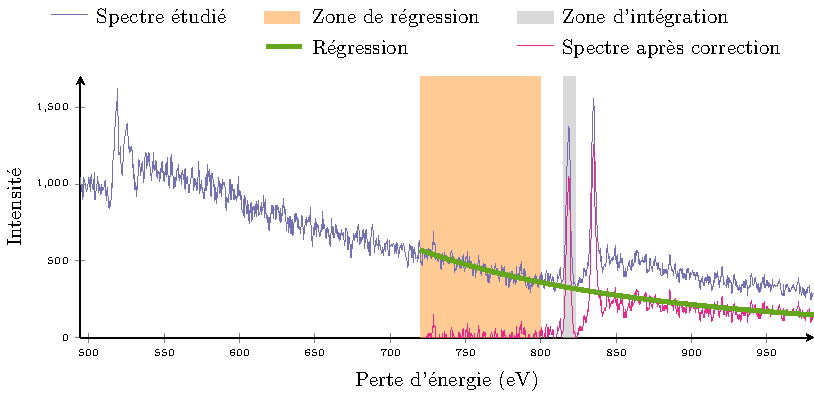
\includegraphics[]{img/chapitre2/figure11/separation.pdf}}\hspace{1em}
        \subfigure[\label{fig-carto-separation-b}]{
            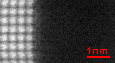
\includegraphics[width=5cm]{img/chapitre2/figure11/regression-sc.png}}
        \caption{Illustration de la méthode de cartographie par séparation de composantes spectrales. \protect\subref{fig-carto-separation-a} régression pour une position particulière. Une régression exponentielle est effectuée sur la zone de régression, puis est soustraite au spectre pour obtenir le spectre corrigé. L'abondance est finalement calculée en intégrant le spectre autours du pic d'intérêt. \protect\subref{fig-carto-separation-b} résultat en effectuant cette action sur tous les pixels (l'élément cartographié est $\mathrm{La-M}_{4, 5}$). A noter que les paramètres de la régression dépendent de la position spatiale.
            \protect\label{fig-carto-separation}}
    \end{figure*}

    \subsection{Cartographie par démélange}

    Nous l'avons dit plus haut, l'imagerie \gls{eels} est un cas particulier d'imagerie hyperspectrale. L'analyse de telles données consiste également à cartographier l'abondance d'un élément particulier dans une scène (une prise de vue aérienne, par exemple, on parle alors de \emph{remote sensing}). Une hypothèse classique consiste à considérer la zone étudiée comme une mixture de peu d'éléments, si bien que le spectre observé en une position spatiale est un mélange de spectres élémentaires. Le problème de cartographie consiste alors à estimer conjointement les spectres élémentaires et leur proportion pour chaque position spatiale. Ce problème inverse est appelé \emph{démélange hyperspectral}~\cite{bioucas2012hyperspectral} (ou unmixing). Puisque l'estimation conjointe des paramètres nécessite la résolution d'un problème non-convexe, on lui préfère une résolution sous-optimale mais convexe. Les spectres élémentaires sont alors estimés en premier lieu (à l'aide d'algorithmes comme VCA~\cite{nascimento2005vertex} ou SISAL~\cite{bioucas2009variable}), puis les cartes d'abondance sont restituées a posteriori (l'algorithme SUNSAL~\cite{bioucas2010alternating} est un exemple d'algorithme pour cette seconde étape).

    Cette technique a été appliquée avec succès en imagerie EELS~\cite{dobigeon2012spectral, Dobigeon_ELSEVIER_2016} et est prometteuse pour analyser efficacement les données \gls{eels}.


    %
    \section{L'acquisition d'échantillons sensibles : problématiques et stratégies}\label{sec-ech-sensibles}

    \paragraph{Problématique des échantillons sensibles} Pour améliorer la qualité de l'acquisition (et par là même celle de son exploitation), l'expérimentateur doit augmenter la dose totale d'électrons délivrée à chaque position de l'échantillon. Pour cela, il peut agir sur la vitesse des électrons du faisceau ou sur la durée d'exposition par position spatiale. Cependant, augmenter la dose accroît la détérioration subie par l'échantillon~\cite{egerton2004radiation}. Cela est particulièrement problématique pour les échantillons sensibles tels que les tissus biologiques. \emph{Il en résulte un compromis entre une qualité d'image satisfaisante et la préservation de l'échantillon d'étude}. Pour illustrer cela, un exemple d'échantillon détérioré par une concentration trop importante d'énergie est donné à la \cref{fig-echantillon-deteriore}. Dès lors, \emph{des stratégies sont nécessaires afin d'améliorer la qualité du spectre-image sans augmenter la quantité d'énergie délivrée à l'échantillon}.

    \begin{figure}[t]
        \centering
        \subfigure[\label{fig-echantillon-deteriore-a}]{%
            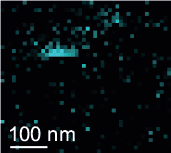
\includegraphics[width=0.3\textwidth]{img/chapitre2/figure12/sequentialScan.png}}\hspace{1em}
        \subfigure[\label{fig-echantillon-deteriore-b}]{%
            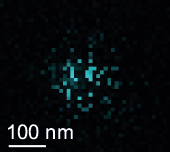
\includegraphics[width=0.3\textwidth]{img/chapitre2/figure12/randomScan.png}}
        \caption{\protect\subref{fig-echantillon-deteriore-a} Exemple d'échantillon détérioré par un faisceau trop énergétique. L'acquisition est réalisée ligne par ligne en commençant au pixel supérieur gauche. \`A un certain stade de l'acquisition, une structure apparaît. Celle-ci est censée être ronde, mais au lieu de cela, plus rien n'est observée quelques lignes après le début du signal. En effet, l'énergie du faisceau était trop grande et la structure a été détruite. A cela s'ajoute que l'acquisition ligne par ligne accumule trop d'énergie dans des positions successives, ce qui dégrade encore davantage l'échantillon. \protect\subref{fig-echantillon-deteriore-b} Acquisition d'une structure semblable avec une acquisition aléatoire et une énergie par pixel égale. La structure n'est pas détériorée puisque l'énergie est davantage répartie au cours de l'échantillonnage.
            \protect\label{fig-echantillon-deteriore}}
    \end{figure}

    \paragraph{Acquisition ligne par ligne v.s. aléatoire} Une première solution pour réduire la détérioration de l'échantillon à énergie fixée consiste à échantillonner de manière aléatoire uniforme. En effet, l'acquisition ligne par ligne est très simple à implémenter, mais cette modalité détériore particulièrement l'échantillon puisqu'elle accumule des doses d'énergie sur des pixels voisins. Pour pallier ce problème, des travaux récents ont mis au point un obturateur coupant le faisceau au cours de l'acquisition~\cite{beche2016development, tararan2016random}, rendant le chemin d'acquisition hautement paramétrable. Ainsi, un parcours aléatoire de l'échantillon permet de visiter successivement des positions spatiales éloignées, ce qui répartie la dose d'électron sur l'ensemble de l'échantillon. Cela est mis en évidence en \cref{fig-echantillon-deteriore-b} puisque la structure spatiale est totalement visible pour une acquisition aléatoire tandis que l'échantillonnage ligne par ligne détruit la structure (cf \cref{fig-echantillon-deteriore-a}). Cette technique permet donc d'augmenter l'énergie délivrée à l'échantillon pour une détérioration égale, et donc d'améliorer la qualité de l'image.

    \paragraph{Correction de la dérive de l'échantillon} Comme expliquée en \cref{sec-prop-eels}, l'échantillon n'est pas stable au cours de l'acquisition puisque des gradients de température et des mouvements d'air le font dériver. Dans le cas d'une acquisition ligne par ligne, cela se manifeste par une déformation du réseau atomique, comme le montre la \cref{fig-drift}. Dans le cas d'un échantillonnage aléatoire, cela détériore grandement la résolution spatiale, particulièrement pour les échantillons à échelle atomique. Pour corriger cela, une méthode consiste à extraire $N$ sous-acquisitions partielles de l'acquisition aléatoire complète. Chacune de ces acquisition partielle est alors complété indépendamment à l'aide d'une méthode de reconstruction (cf \cref{ch-chapter_2}) et le mouvement de l'échantillon est estimé. Les échantillons associés à chaque sous-acquisition sont alors recalés pour compenser la dérive. Cette méthode est appelée \emph{multi-trame} et a été implémentée avec succès en imagerie \gls{haadf} et \gls{eels}~\cite{zobelli2019spatial}. Cette méthode améliore sensiblement la qualité de l'image.

    \paragraph{Débruitage v.s. inpainting} La méthode la plus simple pour limiter la détérioration de l'échantillon consiste à réduire la dose d'électron et à débruiter les données en post-traitement. Cependant, réduire l'exposition peut être d'intérêt limité puisque l'acquisition est trop dégradée pour atteindre des performances de débruitage satisfaisantes, tout particulièrement dans le cas où les structures analysées sont fines.
    %
    Si bien qu'une alternative consiste à conserver une dose d'électrons élevée, mais à ne visiter que peu de positions spatiales. Cette technique rendue possible par l'acquisition aléatoire ne fournie pourtant qu'une image partielle et une méthode de reconstruction est nécessaire afin de compléter les pixels manquants. A cette fin, le \cref{ch-chapter_2} fera le point sur les techniques de reconstruction d'image et sur leur utilisation en microscopie. Cette approche est un domaine de recherche très actif en microscopie \gls{stem}~\cite{beche2016compressed,stevens2014potential} et \gls{sem}~\cite{anderson2013sparse} entre autres.
    %
    Les deux stratégies proposées ont à la fois des avantages et des inconvénients. D'une manière générale, une acquisition à faible dose fournit des informations spatiales plus riches tandis que les données partiellement acquises ont un contenu spectral plus riche. Déterminer quelle approche est la meilleure n'est pas trivial et des études récentes ont comparées ces deux approches~\cite{trampert2018ultramicroscopy} en se basant sur des expériences réalisées sur des images synthétiques et réelles.
    
    % Parler aussi des travaux concernant le choix d'un bon chemin d'acquisition. -> chap 2



    \section{\'Etat des installations au \glsentryshort{lps}}

    Avant d'étudier les techniques de reconstruction dans le cadre du traitement de l'image, il convient de faire le point sur les techniques déjà testées au sein de l'équipe STEM du \gls{lps}.

    La position de la sonde électronique sur l'échantillon est pilotée par des bobines magnétiques. Le mode d'acquisition aléatoire a été implémenté à l'aide d'un module de balayage basé sur FPGA (Field-Programmable Gate Array) contrôlant directement les bobines de balayage~\cite{zobelli2019spatial}. L'ordre des pixels est mélangé aléatoirement dans une phase initiale, puis ce chemin aléatoire est chargé dans un générateur de chemin. Pour chaque pixel, le faisceau illumine l’échantillon uniquement pendant le temps requis pour l’acquisition du signal, temps durant lequel la caméra est en mode d’exposition. Le faisceau d’électrons est coupé pendant le déplacement grâce à un obturateur de faisceau électrostatique. Ce système est actuellement installé sur deux microscopes \gls{stem} :
    \begin{itemize}
        \item un VG-HB501 avec une résolution de l’ordre du nm (cf. \cref{fig-LPS-micro-a}),
        \item un Nion UltraSTEM 200 équipé d’un correcteur d’aberrations sphériques qui permet d’atteindre une résolution de l’ordre de 0,1 nm (cf. \cref{fig-LPS-micro-b}).
    \end{itemize}

    \begin{figure*}
        \centering  % 0.8, 0.5
        \subfigure[\label{fig-LPS-micro-a}]{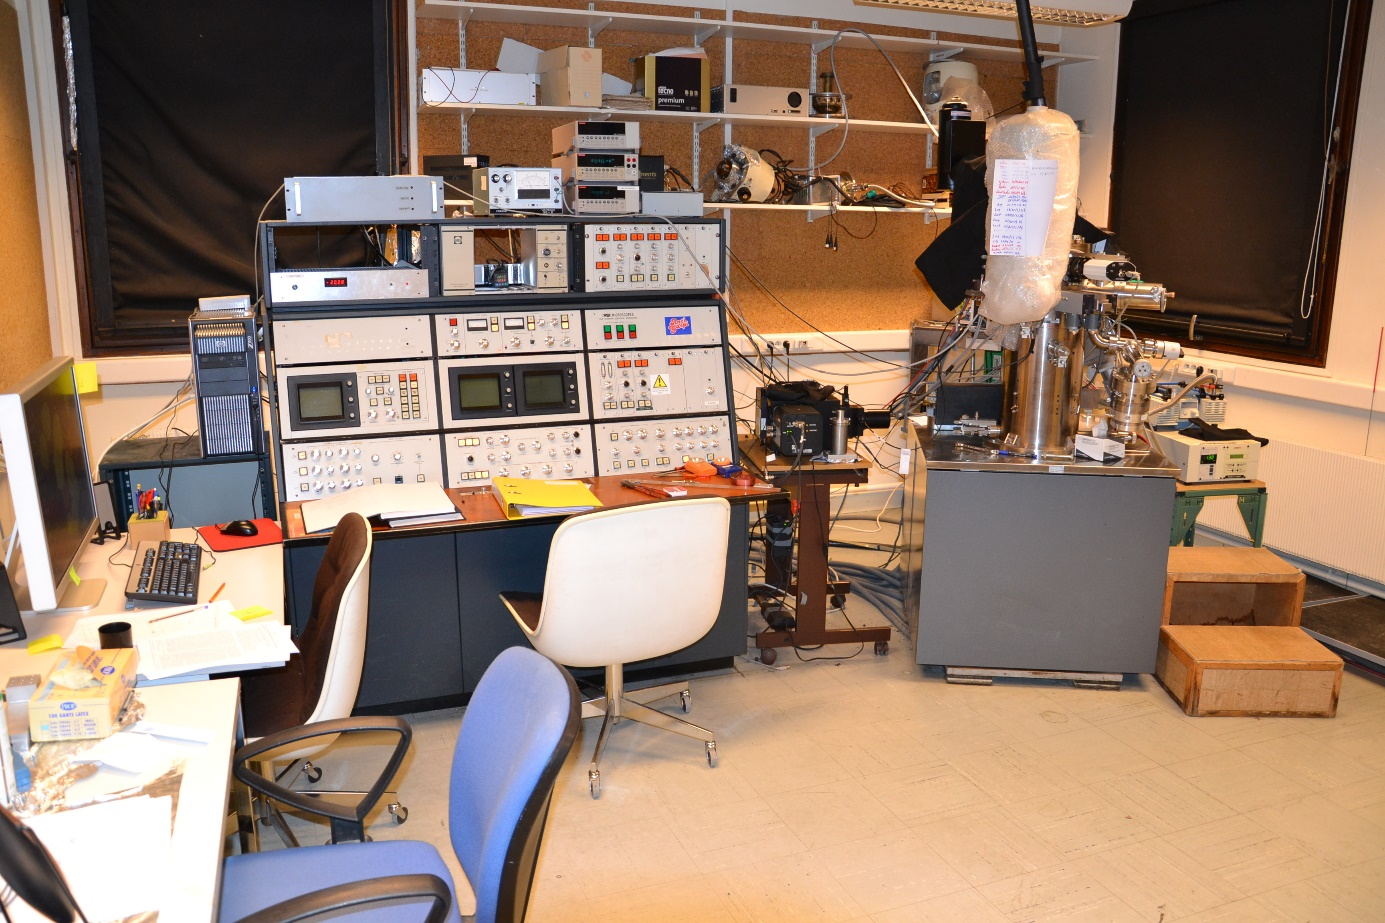
\includegraphics[width=0.5\textwidth]{img/chapitre2/figure13/VG.jpg}}
        \hspace{1em}
        \subfigure[\label{fig-LPS-micro-b}]{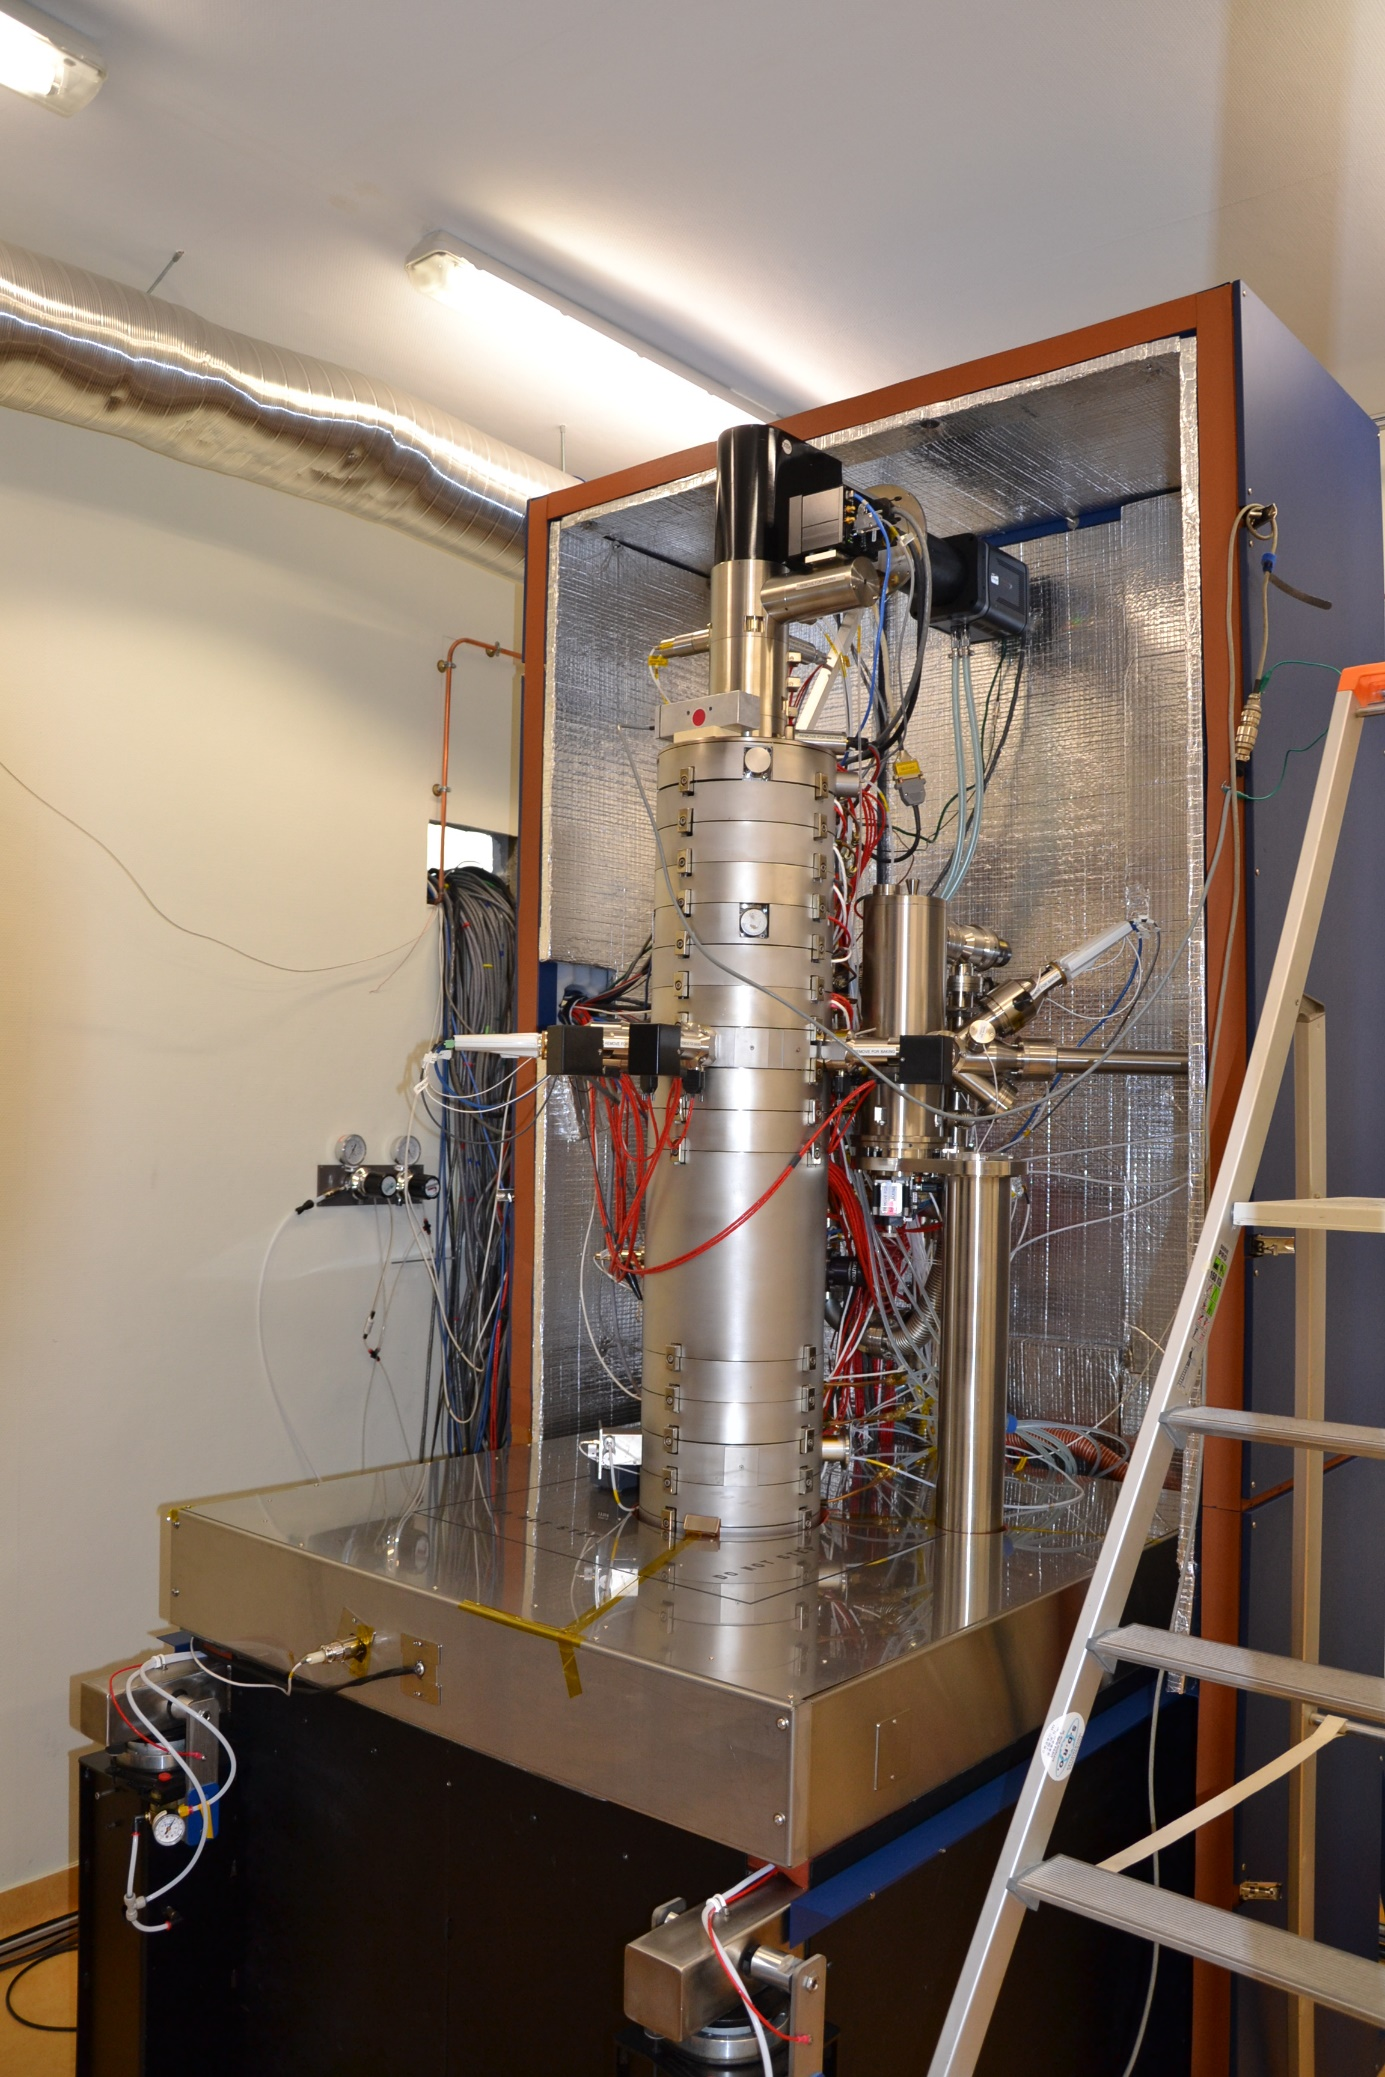
\includegraphics[width=0.4\textwidth]{img/chapitre2/figure13/NION.jpg}}
        \caption{Microscopes en service au \gls{lps} sur lesquels le mode d'acquisition aléatoire est implémenté. \subref{fig-LPS-micro-a} VG-HB501. \subref{fig-LPS-micro-b} Nion UltraSTEM 200.
            \protect\label{fig-LPS-micro}}
    \end{figure*}

    Se basant sur ce système, une approche multi-frame corrigeant la dérive de l'échantillon et améliorant la qualité de l'image a été envisagée~\cite{zobelli2019spatial}. Cependant, cette technique est encore très peu utilisée car lourde d'un point de vue expérimental. En pratique, la dérive est limitée en laissant l'échantillon se stabiliser après insertion dans le microscope et en s'assurant que l'acquisition soit suffisamment rapide. Enfin, dans le cas d'un échantillonnage ligne par ligne où l'échantillon dérive uniformément, il est également possible de corriger le défaut par déformation géométrique du réseau.

    % Figure

    Le débruitage du spectre-image a été utilisé pour améliorer la qualité de l'acquisition, en particulier pour des temps d'exposition faibles ou des échantillons sensibles.  La technique la plus couramment utilisée en spectroscopie \gls{eels} consiste à appliquer une \gls{pca} et à ne conserver que les composantes les plus puissantes (cette technique a déjà été présentée aux \crefrange{sec-prop-eels}{sec-exploitation-eels}). D'autres approches ont été testées lors d'un stage étudiant en 2019, mais elles restent encore très peu utilisées.

    Enfin, les techniques de reconstruction sont encore assez marginales dans l'équipe et ont été utilisées en cathodoluminescence~\cite{zobelli2019spatial} et dans le cadre de cette thèse (échantillon biologique sur VG, NNO/LAO sur UltraStem). Des essais ont été menés \textit{in situ} (c'est-à-dire en chauffant l'échantillon et en observant l'évolution), mais les résultats sont encore peu probants.






%    \begin{subappendices}
%        \section{Quelques notions sur l'\glsentryshort{pca}} % (fold)
%        \label{app-pca}
%
%            Normal equation
%            \begin{equation}
%            \label{eq:normal}
%                \sum_{n=1}^{N} 1 / n \approx \ln(N)
%            \end{equation}
%
%            full width equation
%
%            \begin{fullwidth}
%                \begin{equation}
%                \label{eq:normal}
%                    \sum_{n=1}^{N} 1 / n \approx \ln(N)
%                \end{equation}
%            \end{fullwidth}
%
%            \subsection{subsection name} % (fold)
%            \label{app:sub:subsection_name}
%
%            % subsection subsection_name (end)
%
%        % section section_name (end)
%    \end{subappendices}

% chapter chapter_1 (end)
